\documentclass[11pt,a4paper]{ctexart}
\usepackage{amsmath, amsthm, amssymb, graphicx,mathrsfs}
\usepackage{geometry}
\usepackage[colorlinks=true,hidelinks]{hyperref} % 目录添加超链接
\geometry{left=1.24cm, right=1.24cm, top=1.91cm, bottom=1.91cm}
\title{现代控制理论}
\author{W·D·Gaster}

\renewcommand{\d}{{\rm d}}
\newcommand{\e}{{\rm e}}
\renewcommand{\j}{{\rm j}}


\usepackage{booktabs}
\usepackage{unicode-math}   % 添加\symbfit以实现加粗斜体命令
\newcommand{\bm}{\symbfit}

\usepackage{pifont} %使用带圈数字序号
\usepackage{enumitem}%自定义列表序号

\graphicspath{{figures/}} % 指定图片路径
\usepackage{float}

\begin{document}

\maketitle
\thispagestyle{empty}
\newpage

\tableofcontents
\thispagestyle{empty}
\newpage

\setcounter{page}{1}
    
现代控制理论中的运用状态空间法描述输入-状态-输出诸变量间的因果关系，不但反映了系统的输入输出外部特性，而且揭示了系统内部的结构特性，
是一种既适用于单输入单输出系统又适用于多输入多输出系统，既可用于线性定常系统又可用于线性时变系统的有效分析和综合方法。

\section{系统的状态空间表达式}
    \subsection{状态空间的基本概念}
        状态：系统在时间域中的行为或运动信息的集合。

        状态变量：确定系统状态的一组独立的数目最小的变量。将状态变量看做向量的分量，则该向量称为状态向量。$\bm{x}(t)=[x_1(t),x_2(t),\cdots,x_n(t)]^T$

        状态空间：以n个状态变量作为基底组成的n维空间。

        状态轨线：系统在任一时刻的状态在状态空间中用一个点表示。时间的推移描绘出的一条轨迹。

        线性连续系统的状态空间表达式：
        \[
        \begin{cases}
            \bm{\dot{x}}(t)=\bm{A}(t)\bm{x}(t)+\bm{B}(t)\bm{u}(t)\\
            \bm{y}(t)=\bm{C}(t)\bm{x}(t)+\bm{D}(t)\bm{u}(t)\\
        \end{cases}
        \]
        其中，$\bm{x}(t)$是系统的状态向量，$\bm{u}(t)$是系统的控制输入向量，$\bm{A}$是系统的量测输出向量，
        $\bm{A}$称为系统矩阵或状态矩阵，$\bm{B}$为控制矩阵或输入矩阵，$\bm{C}$为观测矩阵或输出矩阵，$\bm{D}$为前馈矩阵。

        当系统矩阵都是与时间无关的常值函数矩阵时，系统为线性连续定常系统，状态空间可以表示为：
        \[
        \begin{cases}
            \bm{\dot{x}}(t)=\bm{A}\bm{x}(t)+\bm{B}\bm{u}(t)\\
            \bm{y}(t)=\bm{C}\bm{x}(t)+\bm{D}\bm{u}(t)\\
        \end{cases}
        \]

        对应的，采样周期为$T$，采样时刻为$kT$的线性离散系统和线性离散定常系统分别为：
        \[
        \begin{cases}
            \bm{x}(k+1)=\bm{G}(k)\bm{x}(k)+\bm{H}\bm{u}(k)\\
            \bm{y}(k)=\bm{C}(k)\bm{x}(k)+\bm{D}(k)\bm{u}(k)\\
        \end{cases}
        \]

        \[
        \begin{cases}
            \bm{x}(k+1)=\bm{G}\bm{x}(k)+\bm{H}\bm{u}(k)\\
            \bm{y}(k)=\bm{C}\bm{x}(k)+\bm{D}\bm{u}(k)\\
        \end{cases}
        \]

        \begin{figure}[H]
            \centering
            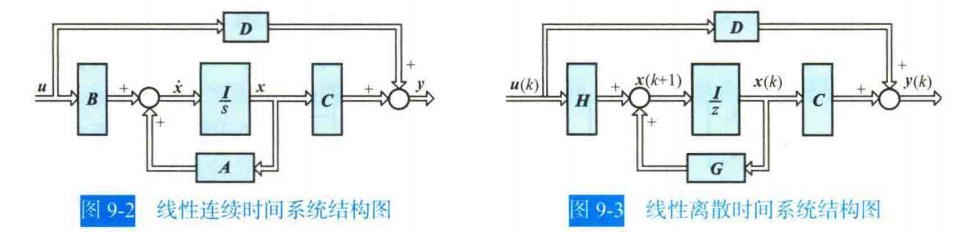
\includegraphics{线性定常系统结构图.png}
            \caption{状态空间表示的系统结构图}
        \end{figure}

    \subsection{建立状态空间表达式的方法}
        \begin{enumerate}
            \item 由系统方框图：
            把系统方框图变换成模拟图，将每个积分器的输出选作一个状态变量$x_i$，对应的输入为$\dot{x}_i$，然后直接写出状态方程和输出方程。
\newpage
            \begin{figure}[H]
                \centering
                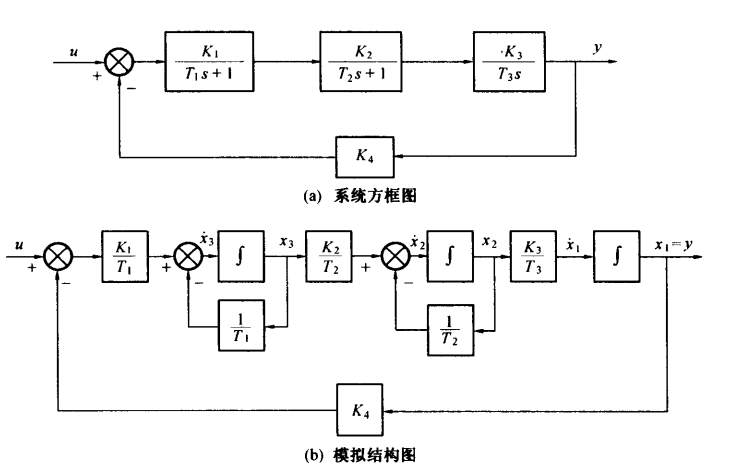
\includegraphics{系统结构图.png}
                \caption{系统模拟结构图}
            \end{figure}
            \item 由系统机理：
            根据物理规律，如电路的基尔霍夫定律或者理论力学的牛顿定律列写方程
            \item 由系统的输入输出关系：            
            将传递函数进行部分分式展开$G(s)=\dfrac{\beta_{n-1}s^{n-1}+\cdots+\beta_1s+\beta_0}{(s-\lambda_1)\cdots(s-\lambda_n)}=\sum\limits_{i=1}^n\dfrac{c_i}{s-\lambda_i}$

            令$X_i(s)=\dfrac{U(s)}{s-\lambda_i}$，则$sX_i(s)-\lambda_iX_i(s)=U(s)$，拉氏逆变换得$\dot{x}_i=\lambda_ix_i+u$，
                
            因此状态方程为$\bm{\dot{x}}=\bm{\Lambda}\bm{x}+[1,1,\cdots,1]^T\bm{u}$，输出方程$y=[c_1,c_2,\cdots,c_n]\bm{x}$

            对于线性定常系统的状态空间表达式，取拉普拉斯变换得：
            \[
            \begin{cases}
                s\bm{\dot{X}}(s)=\bm{A}\bm{X}(s)+\bm{B}\bm{U}(s)\\
                s\bm{Y}(s)=\bm{C}\bm{X}(s)+\bm{D}\bm{U}(s)\\
            \end{cases}
            \]

            代入化简得$\bm{G}(s)=\bm{C}(s\bm{I}-\bm{A})^{-1}\bm{B}+\bm{D}$

            对于离散系统，将脉冲传函写成$G(z)=d+\sum\limits_{i=1}^n\dfrac{k_i}{z-z_i}$，

            令$x_i(z)=\dfrac{u(z)}{z-z_i}$，则有
            \[
            \begin{cases}
                zx_i(z)=z_ix_i(z)+u(z)\\
                y(z)=du(z)+\sum\limits_{i=1}^nk_ix_i(z)
            \end{cases}
            \]

            作 Z 反变换得
            \[
            \begin{cases}
                x_i(k+1)=z_ix_i(k)+u(k)\\
                y(k)=\sum\limits_{i=1}^nk_ix_i(k)+du(k)
            \end{cases}
            \]

            即
            \[
            \begin{cases}
                \bm{x}(k+1)={\rm diag}(z_i)\bm{x}(k)+\begin{bmatrix}1\\ \vdots\\1\end{bmatrix}u(k)\\
                y(k)=[k_1\quad\cdots k_n]\bm{x}(k)+du(k)
            \end{cases}
            \]
            \item 连续系统离散化
            连续系统周期采样且加入零阶保持器得到的等价离散系统系数矩阵有如下关系：
            \[
            \begin{cases}
                \bm{G}(k)=\bm{\Phi}[(k+1)T,kT]=\bm{\Phi}(k+1,k)\\
                \bm{H}(k)=\int_{kT}^{(k+1)T}\bm{\Phi}[(k+1)T,\tau]\bm{B}(\tau)\d\tau\\
                \bm{C}(k)=\bm{C}(t)|_{t=kT}\\
                \bm{D}(k)=\bm{D}(t)|_{t=kT}
            \end{cases}
            \]

            因此线性连续定常系统的离散化模型为
            \[
            \bm{G}=\e^{\bm{A}T}\quad\bm{H}=\bigg(\int_0^T\e^{\bm{A}T}\d t\bigg)\bm{B}
            \]
        \end{enumerate}

        连续系统的零点：
        $rank[s\bm{I}-\bm{A}\quad\bm{B}]<n$的$s$为系统的输入解耦零点；
        $rank\begin{bmatrix}s\bm{I}-\bm{A}\\\bm{C}\end{bmatrix}<n$的$s$为系统的输出解耦零点；
        $rank\begin{bmatrix}s\bm{I}-\bm{A} & -\bm{B}\\\bm{C} & \bm{D}\end{bmatrix}<n+min\{r,m\}$的$s$为系统的传输零点；

        离散系统的零点：
        $rank[s\bm{I}_n-\bm{G}\quad\bm{H}]<n$的$s$为系统的输入解耦零点；
        $rank\begin{bmatrix}s\bm{I}_n-\bm{G}\\\bm{C}\end{bmatrix}<n$的$s$为系统的输出解耦零点；
        $rank\begin{bmatrix}s\bm{I}_n-\bm{G} & -\bm{H}\\\bm{C} & \bm{D}\end{bmatrix}<n+min\{r,m\}$的$s$为系统的传输零点；

    \subsection{代数等价系统}
        \[
        L:\begin{cases}
            \bm{\dot{x}}(t)=\bm{A}\bm{x}(t)+\bm{B}\bm{u}(t)\\
            \bm{y}(t)=\bm{C}\bm{x}(t)+\bm{D}\bm{u}(t)\\
        \end{cases}
        \]
        \[
        L'\begin{cases}
            \bm{\dot{\bar x}}(t)=\bm{\bar A}\bm{\bar x}(t)+\bm{\bar B}\bm{u}(t)\\
            \bm{\bar y}(t)=\bm{\bar C}\bm{\bar x}(t)+\bm{\bar D}\bm{u}(t)\\
        \end{cases}
        \]   
        若存在定常可逆矩阵$\bm{P}$使得$\bm{\bar A}=\bm{PAP^{-1}},\bm{\bar B}=\bm{PB},\bm{\bar C}=\bm{CP^{-1}},\bm{\bar D}=\bm{D}$
        则称$L$和$L'$为代数等价的。

        代数等价的状态空间模型描述的系统具有完全相同的动态特性。

        相互代数等价的定常系统具有相同的特征多项式、特征方程和极点，具有相同的传递函数或传递函数矩阵，具有相同的输入解耦零点、输出解耦零点和传输零点。
\newpage
\section{系统状态空间表达式的时域分析}
    \subsection{状态转移矩阵}
        对线性时变系统$\bm{\dot{x}}(t)=\bm{A}(t)\bm{x}(t),\bm{x}(t_0)=\bm{x}_0,t\geqslant t_0$，对式子两端积分得：
        \[
        \displaystyle\bm{x}(t)-\bm{x}_0=\int_{t_0}^t\bm{A}(\tau)\bm{x}(\tau)\d\tau
        \]
        此为Volterra型向量积分方程，可运用逐次逼近法得$\bm{x}(t)=\bm{\Phi}(t,t_0)\bm{x}_0$，其中系统状态转移矩阵
        \[
        \displaystyle\bm{\Phi}(t,t_0)=\bm{I}+\int_{t_0}^t\bm{A}(\tau_1)\d\tau_1+\int_{t_0}^t\bm{A}(\tau_1)\int_{t_0}^{\tau_1}\bm{A}(\tau_2)\d\tau_2\d\tau_1+\cdots
        \]
        \paragraph{状态转移矩阵的性质}
            \begin{itemize}
                \item 自反性：对任意$t$，有$\bm{\Phi}(t,t_0)|_{t=t_0}=\bm{I}$
                \item 微分性：$\dfrac{\d}{\d t}\bm{\Phi}(t,t_0)=\bm{A}(t)\bm{\Phi}(t,t_0)$
                \item 传递性：$\bm{\Phi}(t_2,t_1)\bm{\Phi}(t_1,t_0)=\bm{\Phi}(t_2,t_0)$
                \item 反身性：$\bm{\Phi}^{-1}(t,t_0)=\bm{\Phi}(t_0,t)$
            \end{itemize}
    \subsection{线性系统的响应}
        \subsubsection{线性时变系统}
            \[ 
            \bm{\phi}(t,t_0,x_0,\bm{u})=\bm{\phi}(t,t_0,x_0,0)+\bm{\phi}(t,t_0,0,\bm{u})=\bm{\Phi}(t,t_0)\bm{x}_0+\int_{t_0}^t\bm{\Phi}(t,\tau)\bm{B}(\tau)\bm{u}(\tau)\d\tau
            \]

        \subsubsection{线性定常系统}
            由于线性定常系统的系统矩阵为定常矩阵$\bm{A}$，则状态转移矩阵
            \[
            \bm{\Phi}(t,t_0)=\bm{I}+\int_{t_0}^t\bm{A}(\tau)\d\tau+\dfrac{1}{2!}[\int_{t_0}^t\bm{A}(\tau)\d\tau]^2+\dfrac{1}{3!}[\int_{t_0}^t\bm{A}(\tau)\d\tau]^3+\cdots
            \]

            则$\e^{\int_{t_0}^t\bm{A}(\tau)\d\tau}=\e^{\bm{A}(t-t_0)}$

            当$t_0=0$时，系统的转移矩阵为矩阵$\bm{A}$的矩阵指数函数$\e^{\bm{A}t}=\sum\limits_{k=0}^\infty\dfrac{1}{k!}\bm{A}^kt^k$

            则线性定常系统整体响应为$\displaystyle\bm{\phi}(t,t_0,x_0,\bm{u})=\e^{\bm{A}(t-t_0)}+\int_{t_0}^t\e^{\bm{A}(t-\tau)}\bm{B}\bm{u}(\tau)\d\tau$
        
        \subsubsection{矩阵指数函数的性质}
            \begin{itemize}
                \item $\e^{\bm{A}t}|_{t=0}=\bm{I}$
                \item $\dfrac{\d}{\d t}\e^{\bm{A}t}=\bm{A}\e^{\bm{A}t}=\e^{\bm{A}t}\bm{A}$
                \item $\e^{\bm{A}(t+s)}=\e^{\bm{A}t}\e^{\bm{A}s}$
                \item $(\e^{\bm{A}t})^{-1}=\e^{-\bm{A}t}$
                \item 若$\bm{A}\bm{B}=\bm{B}\bm{A}$，则$\e^{(\bm{A}+\bm{B})t}=\e^{\bm{A}t}\e^{\bm{B}t}$
                \item 若$\bm{P}$为可逆阵，且$\bm{A}=\bm{PJP}^{-1}$时，则$\e^{\bm{A}t}=\bm{P}\e^{\bm{J}t}\bm{P}^{-1}$
            \end{itemize}
        \subsubsection{矩阵指数函数的求解}
            \begin{itemize}
            \item 基于定义用级数求解
            \item 基于约当（Jordan）分解
                
            一般矩阵的约当分解为$\bm{A}=\bm{PJP^{-1}}$，其中$\bm{J}={\rm diag}[\bm{J_1\quad J_2\quad\cdots J_l}]$
            \[
            \bm{J}_i=
            \begin{bmatrix}
            \lambda_i & 1 &  \\
                & \ddots & \ddots & \\
                &  & \ddots & 1  \\
                &  &  & \lambda_i\\
            \end{bmatrix}\qquad
            \e^{\bm{J}_i t}=\begin{bmatrix}
            1 & t & \frac{1}{2!}t^2 & \cdots & \frac{1}{(p_i-1)!}t^{p_i-1}\\
            0 & 1 & t & \cdots & \frac{1}{(p_i-2)!}t^{p_i-2}\\
            \vdots & \vdots & \vdots & \ddots & \vdots \\
            0 & 0 & 0 & \cdots & t\\
            0 & 0 & 0 & \cdots & 1\\
            \end{bmatrix}
            e^{\lambda_it}
            \]

            则$\e^{\bm{A}t}=\bm{P}{\rm diag}[\e^{\bm{J_1}t}\quad\e^{\bm{J_2}t}\quad\cdots\e^{\bm{J_l}t}]\bm{P}^{-1}$


            \item 利用拉氏变换法
                
            对于$\bm{\dot{x}}=\bm{Ax},\bm{x}(0)=\bm{x}_0$，取拉氏变换得$s\bm{X}(s)=\bm{AX}(s)+\bm{x}(0)$

            得$\bm{X}(s)=(s\bm{I}-\bm{A})^{-1}\bm{x}(0)$

            进行拉式逆变换得$\bm{x}(t)=\mathscr{L}^{-1}[(s\bm{I}-\bm{A})^{-1}\bm{x}(0)]=\bm{\Phi}(t)\bm{x}(0)$

            于是$\e^{\bm{A}t}=\mathscr{L}^{-1}[(s\bm{I}-\bm{A})^{-1}]$
            \item 利用凯莱-哈密顿（Cayley-Hamilton）定理计算
                
            凯莱-哈密顿定理：若矩阵的特征方程为$s^n+a^{n-1}s^{n-1}+\cdots+a_0=0$，则$\bm{A}^n+a^{n-1}\bm{A}^{n-1}+\cdots+a_0\bm{I}=0$

            因此，$\e^{\bm{A}t}=\alpha_0(t)\bm{I}+\alpha_1(t)\bm{A}+\cdots+\alpha_{n-1}(t)\bm{A}^{n-1}$

            其中系数$\alpha_i(t)$如下
            \begin{itemize}
                \item 当$\bm{A}$的特征值互异时，
                \[
                \begin{bmatrix}
                    \alpha_0(t)\\\alpha_1(t)\\\vdots\\\alpha_{n-1}(t)
                \end{bmatrix}=
                \begin{bmatrix}
                    1 & \lambda_1 & \lambda_1^2 & \cdots & \lambda_1^{n-1}\\
                    1 & \lambda_2 & \lambda_2^2 & \cdots & \lambda_2^{n-1}\\
                    \vdots & \vdots & \vdots & \ddots & \vdots \\
                    1 & \lambda_n & \lambda_n^2 & \cdots & \lambda_n^{n-1}\\
                \end{bmatrix}
                \begin{bmatrix}
                    \e^{\lambda_1t}\\ \e^{\lambda_2t}\\ \cdots \\ \e^{\lambda_nt} \\
                \end{bmatrix}
                \]
                \item 当$\bm{A}$具有重特征值但为循环阵（行向量的每个元素都是前一个行向量各元素依次右移一个位置得到的结果），若$\lambda_1$为三重特征值，$\lambda_2$为二重特征值
                \[
                \begin{bmatrix}
                    \alpha_0(t)\\\alpha_1(t)\\\alpha_2(t)\\\alpha_3(t)\\\alpha_4(t)\\\alpha_5(t)\\\vdots\\\alpha_{n-1}(t)\\
                \end{bmatrix}=
                \begin{bmatrix}
                    0 & 0 & 1 & 3\lambda_1 & \cdots & \frac{(n-1)(n-2)}{2!}\lambda_1^{n-3}\\
                    0 & 1 & 2\lambda_1 & 3\lambda_1^2 & \cdots & \frac{n-1}{1!}\lambda_1^{n-2}\\
                    1 & \lambda_1 & \lambda_1^2 & \lambda_1^3 & \cdots & \lambda_1^{n-1}\\
                    0 & 1 & 2\lambda_2 & 3\lambda_2^2 & \cdots & \frac{n-1}{1!}\lambda_2^{n-2}\\
                    1 & \lambda_2 & \lambda_2^2 & \lambda_2^3 & \cdots & \lambda_2^{n-1}\\
                    1 & \lambda_3 & \lambda_3^2 & \lambda_3^3 & \cdots & \lambda_3^{n-1}\\
                    \vdots & \vdots & \vdots & \vdots & \ddots & \vdots \\
                    1 & \lambda_{n-3} & \lambda_{n-3}^2 & \lambda_{n-3}^3 & \cdots & \lambda_{n-3}^{n-1}\\
                \end{bmatrix}
                \begin{bmatrix}
                    \frac{1}{2!}t^2\e^{\lambda_1t}\\ 
                    \frac{1}{1!}t\e^{\lambda_1t} \\ 
                    \e^{\lambda_1t} \\ 
                    \frac{1}{1!}t\e^{\lambda_2t} \\ 
                    \e^{\lambda_2t}\\ 
                    \e^{\lambda_3t}\\
                    \vdots \\ 
                    \e^{\lambda_{n-3}t} \\
                \end{bmatrix}
                \]
            \end{itemize}
            \end{itemize}
    \subsection{离散系统状态空间时域分析}
        \begin{itemize}
        \item 迭代法：$\bm{x}(k)=\bm{G}^n\bm{x}_0+\sum\limits_{i=0}^{k-1}\bm{G}^{i}\bm{H}\bm{u}(k-i-1)$
        
        矩阵形式为：
        \[
        \begin{bmatrix}\bm{x}(1)\\\bm{x}(2)\\\vdots\\\bm{x}(k)\end{bmatrix}=\begin{bmatrix}\bm{G}\\\bm{G}^2\\\vdots\\\bm{G}^k\end{bmatrix}\bm{x}_0+
        \begin{bmatrix}\bm{H} & 0 & \cdots & 0\\\bm{GH} & \bm{H} & \cdots & 0\\\vdots & \vdots & \ddots & \vdots\\\bm{G^{k-1}H} & \bm{G^{k-2}H} & \cdots & \bm{H}\end{bmatrix}\begin{bmatrix}\bm{u}(0)\\\bm{u}(1)\\\vdots\\\bm{u}(k-1)\end{bmatrix}
        \]

        状态转移矩阵$\bm{\Phi}(k)=\bm{G}^k$
        \begin{itemize}
            \item $\bm{\Phi}(k+1)=\bm{G\Phi}(k)$
            \item $\bm{\Phi}(k-l)=\bm{\Phi}(k-m)\bm{\Phi}(m-l)$
            \item $\bm{\Phi}^{-1}(k)=\bm{\Phi}(-k)$
        \end{itemize}
        \item Z 变换法：对$\bm{x}(k+1)=\bm{G}(k)\bm{x}(k)+\bm{H}\bm{u}(k)$两边取 Z 变换得
        
        $z\bm{X}(z)-z\bm{X}(0)=\bm{GX}(z)+\bm{Hu}(z)$
        
        则$\bm{X}(z)=(z\bm{I}_n-\bm{G})^{-1}z\bm{X}(0)+(z\bm{I}_n-\bm{G})^{-1}\bm{Hu}(z)$

        反 Z 变换得$x(k)=\mathscr{Z}^{-1}[(z\bm{I}_n-\bm{G})^{-1}z\bm{X}(0)]+\mathscr{Z}^{-1}[(z\bm{I}_n-\bm{G})^{-1}\bm{Hu}(z)]$
        \end{itemize}
\newpage
\section{系统的能控性和能观性}
    \subsection{能控性及判定}
        \subsubsection{连续系统能控性的定义}
            系统输入$\bm{u}(t)$控制状态向量$\bm{x}(t)$的能力。

            {\setlength{\parindent}{0pt}\textbf{能控状态}}

            如果对取定初始时刻$t_0$的状态$\bm{\bar x}$，存在一时刻$t_1\geqslant t_0$和一个无约束的容许控制$\bm{u}(t)$，
            使得在这个控制作用下系统由$\bm{\bar x}$触发的运动轨线经过时间$t_1-t_0$后转移到$\bm{x}(t_1)=0$，则称$\bm{\bar x}$为系统的一个能控状态。

            如果状态空间中的所有非零状态都是在$t_0$时刻的能控状态，则称此系统在$t_0$时刻完全能控。
            
            如果对于任意$t_0\in[T_1,T_2]$，系统均是在$t_0$时刻为能控的，则称系统在区间$[T_1,T_2]$上是完全能控的。

            {\setlength{\parindent}{0pt}\textbf{能达状态}}

            如果对取定初始时刻$t_0$的零初始状态$\bm{x}(t_0)=0$，存在一时刻$t_1\geqslant t_0$和一个无约束的容许控制$\bm{u}(t)$，
            使得在这个控制作用下系统由$\bm{x}_0$触发的运动轨线经过时间$t_1-t_0$后转移到$\bm{\bar x}$，则称$\bm{\bar x}$为系统的一个能达状态。

            如果$\bm{\bar x}$对于任意$t_0\in[T_1,T_2]$均为能达的，则称系统在区间$[T_1,T_2]$上是完全能达的或一致能达的。

            如果状态空间中的所有非零状态都是在$t_0$时刻的能达状态，则称此系统在$t_0$时刻完全能达。

            {\setlength{\parindent}{0pt}\textbf{能控状态和能达状态的关系}}
                
            能控状态与控制之间的表达式：$\bm{x}_{+}=-\int_{t_0}^{t_f}\bm{\Phi}(t_0,\tau)\bm{B}(\tau)\bm{u}(\tau)\d\tau$

            能达状态与控制之间的表达式：$\bm{\bar x}=\int_{t_0}^{t_f}\bm{\Phi}(t_f,\tau)\bm{B}(\tau)\bm{u}(\tau)\d\tau=-\bm{\Phi}(t_f,t_0)\bm{x}_{+}$

            这说明能控状态$\bm{x}_{+}$和能达状态$\bm{\bar x}$之间是非奇异的线性变换关系。状态空间的任意一个能控状态必有一个能达状态与之对应，反之亦然。
        \subsubsection{线性连续定常系统能控性的判据}
            \begin{enumerate}
                \item 格拉姆（Gram）矩阵判据：存在$t_1>0$使得Gram矩阵
                \[
                \bm{W}_c(0,t_1)=\int_{0}^{t_1}\e^{-\bm{A}t}\bm{BB^T}\e^{-\bm{A^T}t}\d t
                \]
                为非奇异的。
                \item 能控性矩阵判据：${\rm rank}\bm{Q}_c={\rm rank}[\bm{B}\quad\bm{AB}\quad\cdots\bm{A^{n-1}B}]=n$
                \item PBH秩判据：对系统矩阵$\bm{A}$的所有特征值$\lambda_i$满足${\rm rank}[\lambda_i\bm{I}-\bm{A}\quad\bm{B}]={\rm rank}[s\bm{I}-\bm{A}\quad\bm{B}]=n$
                \item 约当（Jordan）标准型判据：
                \begin{itemize}
                    \item 当特征值两两相异时，对角规范型$\bm{\dot{\bar x}}={\rm diag}[\lambda_i\quad\lambda_2\quad\cdots\quad\lambda_n]\bm{\bar x}+\bm{\bar Bu}$，$\bm{\bar B}$不包含全为零的列。
                    \item 当特征值存在重数时，$\bm{A}={\rm diag}[\bm{J_{l1}}\quad\bm{J_{l2}}\quad\cdots\quad\bm{J_{l_{q_l}}}],
                    \bm{B}=\begin{bmatrix}\bm{b_{l1}}\\ \bm{b_{l2}}\\ \vdots\\ \bm{b_{l_{q_l}}}\end{bmatrix}$，分块矩阵$\bm{b}_{iq_i}$最后一行线性无关
                \end{itemize}
            \end{enumerate}
        \subsubsection{线性连续时变系统能控性的判据}
            \begin{enumerate}
                \item 格拉姆（Gram）矩阵判据：存在$t_1>0$使得Gram矩阵
                \[
                \bm{W}_c(t_1,t_0)=\int_{t_0}^{t_1}\bm{\Phi}(t_1,\tau)\bm{B}(\tau)\bm{B^T}(\tau)\bm{\Phi}^T(t_1,\tau)\d\tau
                \]
                是正定的。
                \item 能控性矩阵判据：（充分条件）假设系统$\bm{A}(t)$和$\bm{B}(t)$的每个元素是n-2和n-1次连续可微的矩阵函数，
                记$\bm{B}_1(t)=\bm{B}(t)$，$\bm{B}_i(t)=-\bm{A}(t)\bm{B}_{i-1}(t)+\bm{\dot B}_{i-1}(t)$，
                若存在某个时刻$t_1>t_0$，使得${\rm rank}\bm{Q}_c(t_1)={\rm rank}[B_1(t)\quad B_2(t)\quad\cdots\quad B_n(t)]=n$    
                \item 基于状态转移矩阵的判据：存在某个时刻$t_1>t_0$，使得矩阵$\bm{\Phi}(t_1,\tau)\bm{B}(\tau)$在$[t_0,t_1]$上行线性独立，
                即对任意n维非零向量$\bm{z}$，都有$\bm z^T\bm{\Phi}(t_1,\tau)\bm{B}(\tau)\neq0$
            \end{enumerate}
            
        \subsubsection{输出能控性}
            描述了控制输入$\bm{u}(t)$对输出量$\bm{y}(t)$的支配能力。
            
            任选控制输入$\bm{u}(t)$使得输出$\bm{y}(t)=\bm{C}\e^{\bm{A}t}\bm{x}_0+\bm{C}\int_0^{t}\e^{\bm{A}(t-\tau)}\bm{Bu}(\tau)\d\tau+\bm{Du}(t)$

            输出能控性判据：
            \begin{itemize}
                \item 基本判据：$m\times l$时变矩阵$\bm{C}\e^{\bm{A}t}\bm{B}+\bm{D}$的m个行彼此线性无关。
                \item 复频域判据：控制$\bm{u}$到输出$\bm{y}$的传递函数矩阵$\bm{D}+\bm{C}(s\bm{I}-\bm{A})^{-1}\bm{B}$的m个行彼此是线性无关的。
                \item 代数判据：输出可控性矩阵${\rm rank}\bm{P}={\rm rank}[\bm{CB}\quad\bm{CAB}\quad\cdots\quad\bm{CA^{n-1}B}\quad\bm{D}]=m$。
            \end{itemize}
        \subsubsection{线性离散系统能控性}
            若对于初始时刻$h\in J_k$和状态空间所有非零状态$\bm{x}_0$，都存在时刻$l\in J_k$和控制$\bm{u}(k)$，使得系统第$l$步状态为零$\bm{x}(l)=0$，则称系统在时刻$h$完全能控。

            若对于初始时刻$h\in J_k$和状态空间所有非零状态$\bm{x}_0$，都存在时刻$l\in J_k$和控制$\bm{u}(k)$，使得系统状态$\bm{x}(l)$可微状态空间中任意非零状态，则称系统在时刻$h$完全能达。

            对于离散系统，可达性矩阵${\rm rank}\bm{Q}_c={\rm rank}[\bm{H\quad GH\quad\cdots\quad G^{k-1}H}]=n$是$(\bm{G,H})$完全能达的充要条件，是完全能控的充分条件。当$\det \bm{Q}_c\neq0$时，系统能达性和能控性等价。

            线性离散系统能控性和能达性等价的充要条件是$\bm{G}(k)$对所有$k\in[h,l-1]$非奇异。如果线性离散系统是连续时间系统离散化得到的，则能控性和能达性必定等价。

            线性定常系统能控性充要条件：${\rm rank}\bm{Q}_c={\rm rank}[\bm{H\quad GH\quad\cdots\quad G^{k-1}H}]=n$。
    \subsection{能观性及判定}
        \subsubsection{能观性的定义}
            能观性是指输出量$\bm{y}(t)$反映状态向量$\bm{x}(t)$的能力。

            如果对初始时刻$t_0$的一个非零的初始状态$\bm{x}_0$，存在一时刻$t_1>t_0$，
            使得区间$[t_0,t_1]$上的系统输出$\bm{y}(t)$可以唯一决定系统的初始状态$\bm{x}_0$，则称状态$\bm{x}_0$在时间$t_0$是能观测的。

            如果状态空间中的所有状态$\bm{x}_0$都是在$t_0$时刻能观测的，则称此系统在$t_0$时刻是完全能观测的。
            
            如果对于任意$t_0\in[T_1,T_2]$，系统均是在$t_0$时刻为能观测的，则称系统在区间$[T_1,T_2]$上是完全能观测的。

            取定初始时刻$t_0$，如果空间中存在至少一个非零状态是不可观测的，则称在$t_0$时刻是不完全能观测的。

        \subsubsection{对偶原理}
            \[
            \Sigma:\begin{cases}
                \bm{\dot{x}}=\bm{Ax}+\bm{Bu}\\
                \bm{y}=\bm{Cx}
            \end{cases}
            \Sigma^*:\begin{cases}
                \bm{\dot{x^*}}=-\bm{A^Tx^*}+\bm{C^Tv}\\
                \bm{z}=\bm{B^Tx^*}
            \end{cases}
            \]
        
            则称系统$\Sigma^*$为系统$\Sigma$的对偶系统，对偶系统的状态向量$\bm{x^*}(t)$称为原系统状态向量$\bm{x}$的协状态。

            系统$\Sigma$的状态转移矩阵和它的对偶系统$\Sigma^*$的状态转移矩阵互为转置逆的关系。

            对偶原理：线性系统$\Sigma$的能控性（能观性）与线性系统$\Sigma^*$的能观性（能控性）等价。

        \subsubsection{线性连续定常系统能观性判据}
        \begin{enumerate}
            \item 格拉姆（Gram）矩阵判据：存在$t_1>0$使得Gram矩阵
            \[
            \bm{W}_o(0,t_1)=\int_{0}^{t_1}\e^{\bm{A}^Tt}\bm{C^TC}\e^{\bm{A}t}\d t
            \]
            为非奇异的。

            \item 能观性矩阵判据：${\rm rank}\bm{Q}_o={\rm rank}\begin{bmatrix}\bm{C}\\ \bm{CA}\\ \vdots\\ \bm{CA}^{n-1}\end{bmatrix}=n$

            \item PBH秩判据：$\bm{A}$没有与$\bm{C}$的所有行相正交的非零右特征向量。对系统矩阵$\bm{A}$的所有特征值$\lambda_i$，
            满足$\bm{A\alpha}=\lambda_i\bm{\alpha},\bm{C\alpha}=0$的特征向量$\bm{\alpha}\equiv\bm{0}$

            \item 约当（Jordan）标准型判据：
            \begin{itemize}
                \item 当特征值两两相异时，对角规范型$\bm{\dot{\bar x}}={\rm diag}[\lambda_i\quad\lambda_2\quad\cdots\quad\lambda_n]\bm{\bar x}\bm{y}=\bm{\bar C\bar x}$，$\bm{\bar C}$
                不包含元素全为零的列。
                \item 当特征值存在重数时，$\bm{A}={\rm diag}[\bm{J_{l1}}\quad\bm{J_{l2}}\quad\cdots\quad\bm{J_{l_{q_l}}}],
                \bm{C}=\begin{bmatrix}\bm{c_{l1}}\\ \bm{c_{l2}}\\ \vdots\\ \bm{c_{l_{q_l}}}\end{bmatrix}$，分块矩阵$\bm{c}_{iq_i}$第一列线性无关。
            \end{itemize}               
        \end{enumerate}
            
        \subsubsection{线性连续时变系统能观性判据}
        \begin{enumerate}
            \item 格拉姆（Gram）矩阵判据：存在$t_1>t_0$使得Gram矩阵
            \[
            \bm{W}_o(t_1,t_0)=\int_{t_0}^{t_1}\bm{\Phi}^T(\tau,t_0)\bm{C}^T(\tau)\bm{C}(\tau)\bm{\Phi}(\tau,t_0)\d\tau
            \]
            是正定的。
            \item 能观性矩阵判据：（充分条件）假设系统$\bm{A}(t)$和$\bm{C}(t)$的每个元素是n-2和n-1次连续可微的矩阵函数，
            记$\bm{C}_1(t)=\bm{C}(t)$，$\bm{C}_i(t)=\bm{C}_{i-1}(t)\bm{A}(t)+\bm{C}_{i-1}(t)$，
            若存在某个时刻$t_1>t_0$使得${\rm rank}\bm{Q}_o(t_1)={\rm rank}[C_1^T(t)\quad C_2^T(t)\quad\cdots\quad C_n^T(t)]=n$
            \item 基于状态转移矩阵的判据：存在某个时刻$t_1>t_0$，使得矩阵$\bm{C}(\tau)\bm{\Phi}(\tau,t_1)$在$[t_0,t_1]$上列线性独立，
            即使得对任意n维非零向量$\bm{z}$，都有$\bm{C}(\tau)\bm{\Phi}(\tau,t_1)\bm{z}\neq0$
        \end{enumerate}
        \subsubsection{线性离散系统的能观性}
            若对于初始时刻$h\in J_k$和状态空间任一非零状态$\bm{x}_0$，都存在时刻$l\in J_k$，可由$[h,l]$上的输出$y(k)$唯一确定$\bm{x}_0$，则称系统在时刻$h$完全能观。

            线性定常系统完全能观的充要条件：${\rm rank}\bm{Q}_o={\rm rank}\begin{bmatrix}\bm{C}\\ \bm{CG}\\ \vdots\\ \bm{CG}^{n-1}\end{bmatrix}=n$
    \subsection{能控规范型和能观规范型}
        \subsubsection{能控规范型}
            引入线性非奇异变换$\bm{\bar x}=\bm{Px},\bm{P}=\bm{Q}_c^{-1}$，导出第一能控规范型
            \[
            \begin{cases}
            \bm{\dot{\hat x}}=\bm{A_c\hat x}+\bm{b_c u}\\
            \bm{y}=\bm{c_c\hat x}
            \end{cases}
            \]
            其中,
            \[
            \bm{A_c}=\begin{bmatrix}
                0 & \cdots & 0 & -\alpha_0 \\
                1 & \cdots & 0 & -\alpha_1 \\
                \cdots &  & \cdots & \cdots \\
                0 & \cdots & 1 & -\alpha_{n-1} \\
            \end{bmatrix},
            \bm{b_c}=\begin{bmatrix}
                1\\0\\ \vdots \\ 0 \\
            \end{bmatrix}
            \bm{c_c}=\bm{cQ_c}=[\bm{cb}\quad\bm{cAb}\quad\cdots\quad\bm{cA^{n-1}b}]
            \]

            定义
            \[
            \bm{P}=[\bm{A^{n-1}b\quad\cdots\quad\bm{Ab}\quad\bm{b}}]\begin{bmatrix}
                1 &  \\
                \alpha_{n-1}  & \ddots \\
                \vdots  & \ddots & \ddots \\
                \alpha_1  & \cdots & \alpha_{n-1} & 1\\
                \end{bmatrix}
            \]
            则在线性非奇异变换将系统转化为第二能控规范型
            \[
            \begin{cases}
            \bm{\dot{\hat x}}=\bm{A_c\hat x}+\bm{b_c u}\\
            \bm{y}=\bm{c_c\hat x}
            \end{cases}
            \]
            其中,
            \[
            \bm{A_c}=\begin{bmatrix}
                0 & 1 & \cdots & 0 \\
                \vdots & \vdots &  & \vdots \\
                0 & 0 & \cdots & 1 \\
                -\alpha_0 & -\alpha_1 & \cdots & -\alpha_{n-1} \\
            \end{bmatrix},
            \bm{b_c}=\begin{bmatrix}
                0\\0\\ \vdots \\ 1 \\
            \end{bmatrix}
            \bm{c_c}=\bm{cP}=[\beta_0\quad\beta_1\quad\cdots\quad\beta_{n-1}]
            \]

            $W(s)=\bm{c_c}(s\bm{I}-\bm{A_c})^{-1}\bm{b_c}=\dfrac{\beta_{n-1}s^{n-1}+\beta_{n-2}s^{n-2}+\cdots+\beta_0}{s^n+\alpha_{n-1}s^{n-1}+\cdots+\alpha_0}$
            
        \subsubsection{能观规范型}
            第一能观规范型

            \[
            \begin{cases}
            \bm{\dot{\tilde x}}=\begin{bmatrix}
                0 & 1 & \cdots & 0 \\
                \vdots & \vdots &  & \vdots \\
                0 & 0 & \cdots & 1 \\
                -\alpha_0 & -\alpha_1 & \cdots & -\alpha_{n-1} \\
            \end{bmatrix}\bm{\tilde{x}}+\begin{bmatrix}\beta_0\\ \beta_1\\ \vdots \\ \beta_{n-1}\end{bmatrix}\bm{u}\\
            \bm{y}=[1\quad0\quad\cdots\quad0]\bm{\tilde{x}}
            \end{cases}
            \]

            第二能观规范型

            \[
            \begin{cases}
            \bm{\dot{\tilde x}}=\begin{bmatrix}
                0 & \cdots & 0 & -\alpha_0 \\
                1 & \cdots & 0 & -\alpha_1 \\
                \vdots &  & \vdots & \vdots \\
                0 & \cdots & 1 & -\alpha_{n-1} \\
            \end{bmatrix}\bm{\tilde{x}}+\begin{bmatrix}\beta_0\\ \beta_1\\ \vdots \\ \beta_{n-1}\end{bmatrix}\bm{u}\\
            \bm{y}=[0\quad\cdots\quad0\quad1]\bm{\tilde{x}}
            \end{cases}
            \]
    \subsection{系统结构分解}
        系统通过代数等价变换，将状态变量分解成四个部分：
        可控可观部分$\bm{\bar x}_{co}$、可控不可观部分$\bm{\bar x}_{c\bar o}$、不可控可观部分$\bm{\bar x}_{\bar c o}$和不可控不可观部分$\bm{\bar x}_{\bar c\bar o}$。
        这样系统可以分为相应的四个子系统，称为系统的结构变换或者规范分解。

        对于线性定常系统$(\bm{A,B,C})$经过线性非奇异变换可变换为$(\bm{\bar A,\bar B,\bar C})$，且$\bm{\bar A}=\bm{PAP^{-1}},\bm{\bar B}=\bm{PB},\bm{\bar C}=\bm{CP^{-1}}$
        则必有${\rm rank}\bm{Q}_c={\rm rank}\bm{\bar Q}_c,{\rm rank}\bm{Q}_o={\rm rank}\bm{\bar Q}_o$

        若连续系统能控或能观，$\lambda_i$为$\bm{A}$的特征值，且$\lambda_i\neq\lambda_j,i\neq j$，则时间离散化系统保持能控或能观的充分条件是：
        对一切满足${\rm Re}|\lambda_i\-\lambda_j|=0$的特征值，有$T\neq\dfrac{2l\pi}{{\rm Im}(\lambda_i-\lambda_j)},l=\pm1,\pm2,\cdots$

        \subsubsection{能控性结构分解}
            求出能控性矩阵的秩${\rm rank}\bm{Q}_c=[\bm{B}\quad\bm{AB}\quad\cdots\quad\bm{A^{n-1}B}]=k$，
            在能控性矩阵中任意选择k个线性无关的列向量$\bm{q_1,q_2,\cdots,q_k}$，再在$\mathbb{R}^n$中任意选取n-k个列向量$\bm{q_{k+1},\cdots,q_n}$，
            使得矩阵$[\bm{q_1\quad\cdots\quad q_k\quad\cdots\quad q_n}]$是可逆的。令$\bm{P^{-1}}=\bm{Q}$即可。
            \[
            \begin{bmatrix}\bm{\dot{\hat x}}_c\\\bm{\dot{\hat x}}_{\bar c}\end{bmatrix}=
            \begin{bmatrix}\bm{\hat A}_c & \bm{\hat A}_{12}\\ 0 & \bm{\hat A}_{\bar c}\end{bmatrix}\begin{bmatrix}\bm{\hat x}_c\\\bm{\hat x}_{\bar c}\end{bmatrix}
            +\begin{bmatrix}\bm{\hat B}_c\\0\end{bmatrix}\bm{u}
            \]

        \subsubsection{能观性结构分解}
            求出能观性矩阵的秩${\rm rank}\bm{Q}_o=\begin{bmatrix}\bm{C}\\ \bm{CA}\\ \vdots \\ \bm{CA^{n-1}}\end{bmatrix}=l$，
            任意选择l个线性无关的行向量$\bm{h_1,h_2,\cdots,h_l}$，再在$\mathbb{R}^n$中任意选取n-l个行向量$\bm{h_{k+1},\cdots,h_n}$，
            使得矩阵$\bm{F}=\begin{bmatrix}\bm{h}_1\\ \bm{h}_2\\ \vdots \\ \bm{h}_n\end{bmatrix}$是可逆的。
            \[
            \begin{bmatrix}\bm{\dot{\hat x}}_o\\\bm{\dot{\hat x}}_{\bar o}\end{bmatrix}=
            \begin{bmatrix}\bm{\hat A}_o & 0\\ \bm{\hat A}_{21} & \bm{\hat A}_{\bar o}\end{bmatrix}\begin{bmatrix}\bm{\hat x}_o\\\bm{\hat x}_{\hat o}\end{bmatrix}
            +\begin{bmatrix}\bm{\hat B}_o\\\bm{\hat B}_{\bar o}\end{bmatrix}\bm{u}
            \]

        \subsubsection{规范分解}
            \[
            \begin{bmatrix}\bm{\dot x}_{co}\\\bm{\dot x}_{c\bar o}\\ \bm{\dot x}_{\bar co}\\\bm{\dot x}_{\bar c\bar o}\end{bmatrix}=
            \begin{bmatrix}\bm{\tilde A}_{co} & 0 & \bm{\tilde A}_{13} & 0\\ 
            \bm{\tilde A}_{21} & \bm{\tilde A}_{c\bar o} & \bm{\tilde A}_{23} & \bm{\tilde A}_{24}\\
            0 & 0 & \bm{\tilde A}_{\bar c o} & 0\\
            0 & 0 & \bm{\tilde A}_{43} & \bm{\tilde A}_{\bar c\bar o}
            \end{bmatrix}
            \begin{bmatrix}\bm{x}_{co}\\\bm{x}_{c\bar o}\\ \bm{x}_{\bar co}\\\bm{x}_{\bar c\bar o}\end{bmatrix}
            +\begin{bmatrix}\bm{\tilde B}_{co}\\0\\0\end{bmatrix}\bm{u}
            \]
            \[
            y=[\bm{\tilde C}_{co}\quad0\quad\bm{\tilde C}_{\bar c o}\quad 0]\bm{x}
            \]
            \begin{figure}[H]
                \centering
                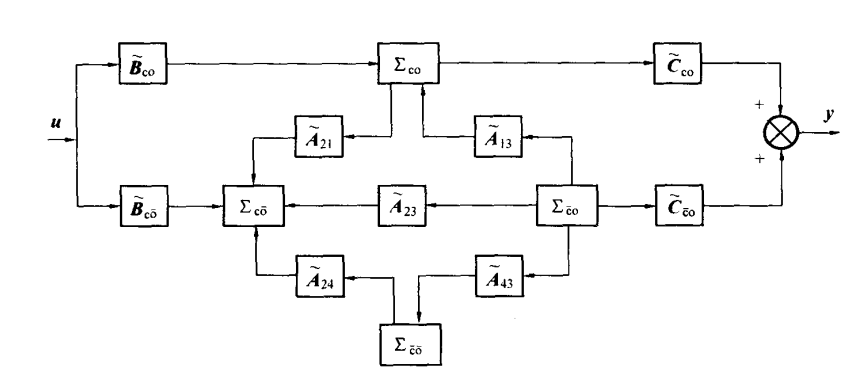
\includegraphics[width=0.7\textwidth]{规范分解结构图.png}
                \caption{系统结构规范分解}
            \end{figure}
\newpage
\section{系统的运动稳定性}
    \subsection{李雅普诺夫（Lyapunov）稳定性的定义}
        设原点为系统的平衡点，则$\forall\varepsilon>0,\exists\delta(\varepsilon,t_0)>0$，使得当$\|\bm{x}_0\|\leqslant\delta(\varepsilon,t_0)$，
        有$\|\bm{x}(t,t_0,\bm{x}_0)\|\leqslant\varepsilon,\forall t\geqslant t_0$，称系统在零平衡点是Lyapunov稳定的。
        当$\delta(t_0,\varepsilon)=\delta(\varepsilon)$，是Lyapunov一致稳定的。

        $\exists\delta(t_0)>0$，当$\|\bm{x}_0\|\leqslant\delta(t_0)$时，$\exists T(\varepsilon,t_0,\bm{x}_0)$，
        对于$\forall t\geqslant t_0+T(\varepsilon,t_0,\bm{x}_0)$有$\|\bm{x}(t,t_0,\bm{x}_0)\|\leqslant\varepsilon$，则称系统的零平衡点是吸引的，
        吸引域为$\{\bm{x}\in\mathbb{R}^n|\|\bm{x}\|\leqslant\delta(t_0)\}$。若$T(\varepsilon,t_0,\bm{x}_0)=T(\varepsilon)$，是一致吸引的。
        若$\delta(t_0)$可以任意大，则称吸引、一致吸引为全局吸引、全局一致吸引。

        若系统的零平衡点是稳定的且为（全局）吸引的，称系统的解对于零平衡点为（全局）渐近稳定的。
        若系统的零平衡点是一致稳定的且（全局）一致吸引的（且方程的解是一致有界的），称为系统对零平衡点是（全局）一致渐近稳定的。

        如果$\forall\varepsilon>0,\exists\delta(\varepsilon)>0,\exists\lambda>0$，当$\|\bm{x}_0\|<\delta$时，
        有$\|\bm{x}(t,t_0,\bm{x}_0)\|<\varepsilon\|\bm{x}_0\|\e^{-\lambda(t-t_0)}$，则称零平衡点是指数稳定的。
        若$\exists k(\delta)>0$，有$\|\bm{x}(t,t_0,\bm{x}_0)\|<k(\delta)\|\bm{x}_0\|\e^{-\lambda(t-t_0)}$，则是全局指数稳定的。
    \subsection{矩阵正定性相关概念}
        若$\forall N>0,\exists R>0$，使得$\|\bm{x}\|>R,V(\bm{x})>N$，即$\lim\limits_{\|\bm{x}\|\rightarrow\infty}V(\bm{x})=\infty$，称$V(\bm{x})$为（径向）无限大的。

        存在无限大性质的正定函数$W(\bm{x})$，使得$V(t,\bm{x})\geqslant W(\bm{x})$（$V(t,\bm{x})\leqslant-W(\bm{x})$）成立且$V(t,0)=0$，则称连续函数$V(t,\bm{x})$具有无限大性质。

        若存在正定函数$W_1(\bm{x})$使得$|V(t,\bm{x})\leqslant W_1(\bm{x})$，则称$V(t,\bm{x})$具有渐减性质或者有无穷小上界。

        函数$\Phi\in C[\mathbb{R}^+,\mathbb{R}^+]$是连续的严格单调上升的函数且有$\Phi(0)=0$，称$\Phi$是K类函数，记为$\Phi\in K$。
        若$\lim\limits_{r\rightarrow\infty}\Phi(r)=+\infty$，称$\Phi$为径向无界K类函数，记为$\Phi\in KR$或$\Phi\in K_{\infty}$

        对于$\|\bm{x}\|\leqslant R$上给定的正定连续函数$W(\bm{x})$，必定存在两函数$\Phi_1,\Phi_2\in K$，使得$\Phi_1(\|\bm{x}\|)\leqslant W(\bm{x})\leqslant\Phi_2(\|\bm{x}\|)$

        对于$\mathbb{R}^n$上给定的无限大正定函数$W(\bm{x})$，必定存在两函数$\Phi_1,\Phi_2\in KR$，使得$\Phi_1(\|\bm{x}\|)\leqslant W(\bm{x})\leqslant\Phi_2(\|\bm{x}\|)$

        设$\Phi,\psi\in K[KR]$，存在常数$k_1,k_2>0$，使得$k_1\Phi\|\bm{x}\|\leqslant\psi(\|\bm{x}\|)\leqslant k_2\Phi\|\bm{x}\|$，则称$\Phi,\psi$具有局部同级增势[全局同级增势]。

        $\bm{Q}(t)$为分段连续的实对称矩阵函数，$\exists M>0,\|\bm{Q}(t)\|\leqslant M$或$\bm{Q}(t)\leqslant M\bm{I}$，则称$\bm{Q}(t)$是一致有界的。
        $\exists m>0,\forall \bm{x}\in\mathbb{R}^n,\bm{x^T Qx}\geqslant m\|\bm{x}\|^2$，则称$\bm{Q}(t)$是一致正定的。
    \subsection{李雅普诺夫（Lyapunov）稳定性定理}
        \subsubsection{稳定性定理}
            对于自治系统，$\bm{x}=\bm{0}$是系统的平衡点，$V$是包含原点的邻域$\Omega$上的连续可微的正定函数，
            若有$\dot V(\bm{x})\leqslant0$，则$\bm{x}=\bm{0}$是Lyapunov稳定的。若有$\dot V(\bm{x})<0$，则$\bm{x}=\bm{0}$是Lyapunov渐进稳定的。
            若$V(\bm{x})$具有无限大性质，则$\bm{x}=\bm{0}$是全局渐进稳定的。

            克拉索夫斯基（Krasovskii）定理：若除零轨线$\bm{x}=\bm{0}$外，没有系统的非零轨线完全包含在$S=\{\bm{x}\in\Omega|\dot{V}(\bm{x})=0\}$中，则原点是渐进稳定的。

            对于非自治系统，$\bm{x}=\bm{0}$是系统的平衡点，$V$是包含原点的邻域$\Omega$上的连续可微的正定函数，
            若$\dot V(\bm{x})\leqslant0$，则$\bm{x}=\bm{0}$是Lyapunov稳定的。
            若$V(t,\bm{x})$是渐减的，则系统平凡解是一致稳定的。若$V(t,\bm{x})$是渐减的连续正定函数，则系统零解是一致渐进稳定的。

            对于离散系统，若$V[\bm{x}(k)]$正定，$\Delta V[\bm{x}(k)]$负半定，且对于任意非零初态的解轨线$\Delta V[\bm{x}(k)]$不恒为零，
            当$\|\bm{x}(k)\|\rightarrow\infty$时$V[\bm{x}(k)]\rightarrow\infty$，则$\bm{x}=0$为大范围渐进稳定。
        \subsubsection{不稳定性定理}
            对于自治系统，在原点的$\Omega$邻域内，若存在连续可微函数$V(\bm{x})$，在$\Omega_1\subset\Omega$内部正定且边界上$V(\bm{x})=0$，且$\dot V(\bm{x})>0$，则平衡点$\bm{x}=\bm{0}$不稳定。
            
            对于非自治系统，在原点的$\Omega$邻域内，存在开集$\Omega_1\subseteq B_r=\{\bm{x}|\|\bm{x}\|\leqslant r\}\subset \Omega $和K类函数$\gamma$，
            存在渐减连续可微函数$V(t,\bm{x})$在$\Omega_1$内正定且边界上$V(t,\bm{x})=0$，且$\dot V(\bm{x})>0$，$V(t,0)=0$，则平衡点$\bm{x}=\bm{0}$不稳定。
        \subsubsection{指数稳定判据}
            若存在$V(t,\bm{x})$满足$\|\bm{x}\|\leqslant V(t,\bm{x})\leqslant K(\alpha)\|\bm{x}\|,x\in S_a=\{\bm{x}:\|\bm{x}\|\leqslant\alpha\},\dot{V}\leqslant-cV(t,\bm{x})$，则零解指数稳定。

            若存在$V(t)\in C[I\times S_a,R]$，及与$\|\bm{x}\|^\lambda$具有局部（全局）同级增势的$\Phi_1,\Phi_2,\psi\in K$，
            使得$\Phi_1(\|\bm{x}\|)\leqslant V(t,\bm{x})\leqslant\Phi_2(\|\bm{x}\|)$且$\dot V\leqslant-\psi(\|\bm{x}\|)$，则零解（全局）指数稳定。
    \subsection{线性系统稳定性判定}
        如果系统的零平衡点稳定，则其他一切平衡点亦稳定。如果零解为渐近稳定的，则必为全局渐近稳定的。
            
        （一致）稳定的充要条件是$\bm{\Phi}(t,t_0)$在$[t_0,\infty)$上（一致）有界。

        渐近稳定的充要条件是$\lim\limits_{t\rightarrow\infty}\|\bm{\Phi}(t,t_0)\|=0$。

        一致渐近稳定的充要条件是$\exists k_1,k_2,\|\bm{\Phi}(t,t_0)\|\leqslant k_1\e^{-k_2(t-t_0)},\forall t\geqslant t_0$。

        如果系统是一致渐近稳定的，则$\bm{P}(t)=\int_t^{\infty}\bm{\Phi^T}(\tau,t)\bm{Q}(\tau)\bm{\Phi}(\tau,t)\d\tau$对任意$t>0$收敛，
        且$\bm{P}(t)$为矩阵微分方程（Lyapunov方程）$-\bm{\dot P}(t)=\bm{P}(t)\bm{A}(t)+\bm{A^T}(t)\bm{P}(t)+\bm{Q}(t),\forall t\geqslant t_0$的唯一解。

        设$\bm{A}(t)$为$[t_0,\infty)$上的一致有界分段连续矩阵，且$\lambda[\bm{A^T}(t)+\bm{A}(t)]<-\delta<0$，则系统一致渐进稳定。

        {\setlength{\parindent}{0pt}\textbf{Lyapunov第一法}}

        线性连续定常系统$\bm{\dot x}=\bm{Ax}$稳定的充要条件是矩阵$\bm{A}$的所有特征值都具有非正实部，且具有零实部的特征值为其最小多项式的单根。
        
        线性连续定常系统$\bm{\dot x}=\bm{Ax}$渐近稳定的充要条件是矩阵$\bm{A}$所有特征值均有负实部，
        或对任意给定的正定对称矩阵$\bm{Q}$，存在正定对称矩阵$\bm{P}$满足Lyapunov矩阵方程$\bm{A^T P}+\bm{PA}=-\bm{Q}$。

        线性离散定常系统$\bm{x}(k+1)=\bm{Gx}(k)$稳定的充要条件是矩阵$\bm{G}$的所有特征根都位于单位圆内，且位于单位圆上的特征值为最小多项式的单根。

        线性离散定常系统$\bm{x}(k+1)=\bm{Gx}(k)$渐进稳定的充要条件是矩阵$\bm{G}$所有特征值均位于单位圆内，
        或对任意给定的正定对称矩阵$\bm{Q}$，存在正定对称矩阵$\bm{P}$满足离散型Lyapunov矩阵方程$\bm{G^T PG-P}=-\bm{Q}$。
    \subsection{构造Lyapunov函数的方法}
        \begin{itemize}
            \item 克拉索夫斯基（Krasovskii）方法：令$\bm{\hat F}(\bm{x})=\bm{F^T}(x)+\bm{F}(\bm{x})$，其中$\bm{F}(x)$是雅可比（Jacobi）矩阵，若其为负定的，则零平衡点是渐近稳定的，
            如果$\|\bm{x}\|\rightarrow\infty$时，Lyapunov函数$V(\bm{x})=\bm{f^T}(\bm{x})\bm{f}(\bm{x})\rightarrow\infty$，则零平衡点是大范围渐近稳定的。
            \item 变量梯度法：$\dot V(\bm{x})=\nabla V^T\bm{\dot x}$，则$\displaystyle V(\bm{x})=\int_0^x\nabla V^T\d x$，
            梯度必须满足广义旋度方程，即$\dfrac{\partial \nabla V_i}{\partial x_j}=\dfrac{\partial \nabla V_j}{\partial x_i}$

            实际应用时通常设
            \[\nabla V=
            \begin{bmatrix}
            a_{11}x_1+a_{12}x_2+\cdots+a_{1n}x_n\\
            a_{21}x_1+a_{22}x_2+\cdots+a_{2n}x_n\\
            \vdots\\
            a_{n1}x_1+a_{n2}x_2+\cdots+a_{nn}x_n\\
            \end{bmatrix}
            \]
        \end{itemize}
\newpage
\section{线性定常系统的状态空间综合}
    \subsection{线性系统的常规控制率}
        对于线性定常系统
        \[
        \begin{cases}
        \bm{\dot{x}}=\bm{Ax}+\bm{Bu}+\bm{Ed}\\
        \bm{y}=\bm{Cx}+\bm{Du}
        \end{cases}
        \]
        其中$\bm{d}$是干扰信号，$\bm{E}$是干扰输入矩阵。

        \subsubsection{状态反馈控制律（直接状态反馈）}
            $\bm{u}=\bm{Kx}+\bm{Gv}$，其中$\bm{K}$状态反馈增益矩阵，$\bm{v}$为外部输入信号，$\bm{G}$为外部输入矩阵

            此时闭环系统为
            \[
            \begin{cases}
            \bm{\dot{x}}=\bm{A_c x}+\bm{B_c v}+\bm{Ed}\\
            \bm{y}=\bm{C_c x}+\bm{D_c v}
            \end{cases}
            \]
            其中$\bm{A_c}=\bm{A}+\bm{BK},\bm{B_c}=\bm{BG},\bm{C_c}=\bm{C}+\bm{DK},\bm{D_c}=\bm{DG}$
            \begin{figure}[H]
                \centering
                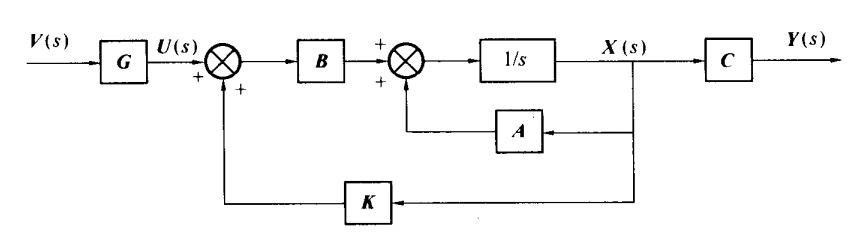
\includegraphics{状态控制反馈.png}
                \caption{$\bm{D}=\bm{0}$时状态控制反馈的方块图}
            \end{figure}

            若输入和输出向量维数相同，且$\bm{G}$非奇异，则状态反馈保持系统的输入解耦零点，保持系统能控性不变，但可能改变能观性。
        \subsubsection{输出反馈控制律}
            $\bm{u}=\bm{Ky}+\bm{Gv}=\bm{KCx}+\bm{Gv}$，其中$\bm{K}$为输出反馈增益矩阵，实际上为一种特殊的状态反馈控制律。

            若输入和输出向量维数相同，且$\bm{G}$非奇异，则状态反馈保持系统的输入解耦零点和输出解耦零点，保持系统能控性和能观性不变。
        \subsubsection{输出动态补偿器}
            \[
            \begin{cases}
            \bm{\dot{z}}=\bm{Fz}+\bm{Hy}+\bm{Lv}\\
            \bm{y}=\bm{Nz}+\bm{My}+\bm{Gv}
            \end{cases}
            \]
            其中$\bm{F,H,L,N,M,G}$适当维数的参数矩阵，$\bm{v}$为外部输入信号，$\bm{z}\in \mathbb{R}^q$为状态向量，$q$为动态补偿器的阶数，$q=0$时不存在动态环节，退化为静态输出反馈控制。

            此时闭环系统为
            \[
            \begin{cases}
            \bm{\dot{x}}=\bm{A_c X}+\bm{B_c v}\\
            \bm{y}=\bm{C_c X}
            \end{cases}
            \]
            其中$\bm{X}=\begin{bmatrix}\bm{x}\\ \bm{z}\end{bmatrix},\bm{A_c}=\begin{bmatrix}\bm{A}+\bm{BMC}\quad\bm{BN}\\ \bm{HC}\quad\bm{F}\end{bmatrix},
            \bm{B_c}=\begin{bmatrix}\bm{BG}\\ \bm{L}\end{bmatrix},\bm{C_c}=[\bm{C}\quad 0]$
            \begin{figure}[H]
                \centering
                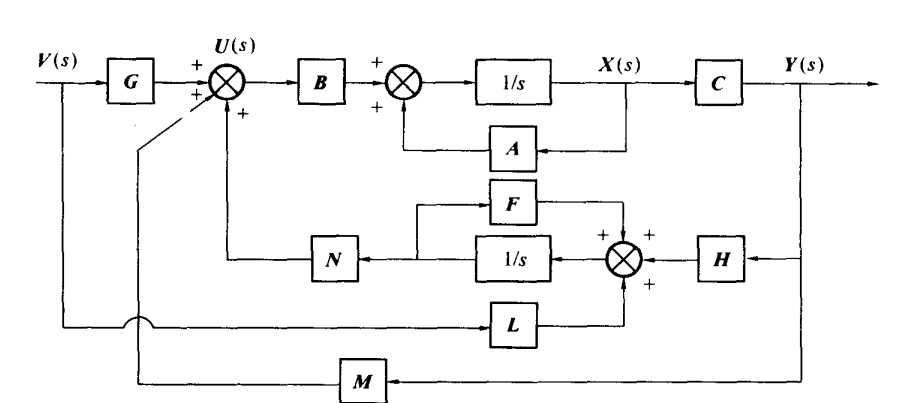
\includegraphics{动态补偿器.png}
                \caption{$\bm{D}=\bm{0}$时动态补偿器的方块图}
            \end{figure}
    \subsection{极点配置}
        通过选定反馈增益矩阵，将闭环系统的极点恰好配置在复平面中所期望的位置，从而达到一定的性能指标的要求。
        
        对于单输入系统$\bm{\dot x}=\bm{Ax}+\bm{b}u$一组期望的闭环特征值$\{\lambda^*_i\}$，确定$1\times n$的反馈增益矩阵$\bm{k}$，
        通过状态反馈$\bm{u}=\bm{kx}+v$使得闭环系统极点满足$\lambda_i(\bm{A}+\bm{bk})=\lambda_i^*$

        充要条件：被控系统完全可控。

        {\setlength{\parindent}{0pt}\textbf{极点配置算法}}

        \newcounter{circled}
        \begin{itemize}[label=\protect\stepcounter{circled}\ding{\the\numexpr191+\value{circled}}]
            \item 计算$\bm{A}$的特征多项式$\det(s\bm{I}-\bm{A})=s^n+a^*_{n-1}s^{n-1}+\cdots+a_1^*s+a_0^*$
            \item 计算由$\{\lambda^*_i\}$决定的特征多项式$a^*(s)=(s-\lambda^*_1)\cdots(s-\lambda^*_n)$
            \item 计算$\bm{\bar k}=[a_0-a_0^*\quad a_1-a_1^*\quad\cdots\quad a_{n-1}-a_{n-1}^*]$
            \item 计算变换阵$\bm{P}=[\bm{A^{n-1}B}\quad\cdots\quad\bm{Ab}\quad\bm{b}]\begin{bmatrix}1&\\a_{n-1}& 1 \\ \cdots &\ddots & \ddots \\a_1 & \cdots & a_{n-1} & 1\end{bmatrix}$
            \item 求$\bm{Q}=\bm{P}^{-1}$
            \item 得出所求的增益阵$\bm{k}=\bm{\bar k Q}$
            \end{itemize}
        \subsection{镇定问题}
        通过设计控制律使闭环系统渐近稳定，即通过控制作用使闭环系统的极点均具有负实部。由于镇定问题只注重系统稳定性，只需将不稳定的极点配置到复平面左半平面即可，可以认为是极点配置问题的一种特殊情形。

        \[
        \begin{cases}
        \bm{\dot{x}}=\bm{Ax}+\bm{Bu}\\
        \bm{y}=\bm{Cx}
        \end{cases}
        \]

        若设计系统的状态反馈控制律$\bm{u}=\bm{Kx}+\bm{Gv}$使得闭环系统能渐近稳定，则称其为系统的一个状态反馈镇定控制律。
        如果一个线性定常系统通过状态反馈控制使系统镇定，则称系统可稳或矩阵对$[\bm{A}\quad\bm{B}]$是可稳的。

        系统可镇定的充要条件是该系统的一切不能控振型，即系统的输出解耦零点，均具有负实部。

        \begin{itemize}
            \item 利用能控性分解的设计方法：
            \begin{itemize}
                \item 将系统进行能控性分解，获得变换矩阵$\bm{P}$以及
                $\bm{\bar A}=\bm{PAP^{-1}}=\begin{bmatrix}\bm{A}_c\quad \bm{A}_{12}\\ \bm{0}\quad\bm{A}_{\bar c}\end{bmatrix},\bm{\bar B}=\bm{PB}=\begin{bmatrix}\bm{B}_c\\ \bm{0}\end{bmatrix}$
                \item 利用极点配置方法求取矩阵$\bm{K}_c$使得矩阵$\bm{A}_c+\bm{B}_c\bm{K}_c$具有一组负实部的特征值
                \item 计算状态反馈镇定律增益矩阵$\bm{K}=[\bm{K}_c\quad\bm{0}]\bm{P}$
            \end{itemize}

            \item 基于Riccati代数方程的设计方法：
            \begin{itemize}
                \item 任取对称正定矩阵$\bm{Q}\in\mathbb{R}^{n\times n}$，求取Riccati代数方程$\bm{A^TP}+\bm{PA}-\bm{PBB^TP}+\bm{Q}=\bm{0}$的唯一对称非负定解，若这样的解不存在则系统不可稳，镇定律不存在。
                \item 计算状态反馈增益矩阵$\bm{K}=-\bm{B^TP}$
            \end{itemize}
        \end{itemize}
        
        {\setlength{\parindent}{0pt}\textbf{定常参考信号的渐进跟踪问题}}

        对于跟定的某一连续信号$\bm{y}_r(t)$，通过状态反馈使得系统输出$\bm{y}(t)$满足$\lim\limits_{t\rightarrow\infty}[\bm{y}(t)-\bm{y}_r(t)]=0$，则称此为渐近跟踪问题。
        首先考虑$\bm{y}_r(t)=\bm{y}_r$的问题。

        经典控制理论中采用PI控制器对误差进行比例积分控制使得系统是无差的。推广到多变量系统中，在误差向量的每一个分量后串入积分器，从而使静态误差的每一个分量都为零。

        记$\displaystyle\bm{q}(t)=\int_0^t\bm{e}(\tau)\d\tau=\int_0^t(\bm{y}(t)-\bm{y}_r)\d\tau$，则有$\bm{\dot q}=\bm{y}(t)-\bm{y}_r$，得增广系统如下：
        \[
        \begin{cases}
        \begin{bmatrix}\bm{\dot{x}}\\ \bm{\dot q}\end{bmatrix}=\begin{bmatrix}\bm{A} & \bm{0}\\ \bm{C} & \bm{0}\end{bmatrix}\begin{bmatrix}\bm{x}\\ \bm{q}\end{bmatrix}
        +\begin{bmatrix}\bm{B}\\\bm{0}\end{bmatrix}\bm{u}
        -\begin{bmatrix}\bm{0}\\\bm{y}_r\end{bmatrix}+\begin{bmatrix}\bm{E}\\\bm{0}\end{bmatrix}\bm{d}\\
        \bm{y}=[\bm{C}\quad\bm{0}]\begin{bmatrix}\bm{x}\\ \bm{q}\end{bmatrix}
        \end{cases}
        \]

        该增广系统的状态反馈控制律$\bm{u}=[\bm{K}_x\quad\bm{K}_q]\begin{bmatrix}\bm{x}\\ \bm{q}\end{bmatrix}=\bm{K_x x}+\bm{K_q q}$
        
        \[
        \bm{u}=\bm{K_x x}+\bm{K_q}\int_0^t[\bm{y}(\tau)-\bm{y_r}]\d\tau
        \]

        设$(\bm{A,B})$能控，则上述增广系统完全能控的充要条件为${\rm rank}\begin{bmatrix}\bm{A}&\bm{B}\\ \bm{C}&\bm{0}\end{bmatrix}=m+n$
    \subsection{状态重构问题}
        为解决系统不完全可观测时无法进行全状态反馈，需要进行重构系统状态，重构核心就是利用原系统可以直接测量的变量作为输入信号，构造系统的输出量$\bm{\bar x}(t)$使得在一定意义下与原系统状态$\bm{x}(t)$等价。
        通常称$\bm{\bar x}(t)$为$\bm{x}(t)$的重构状态或估计状态，称实现状态重构的系统为观测器。
        等价性采用渐近等价的指标，即$\lim\limits_{t\rightarrow\infty}\bm{\tilde x}(t)=\lim\limits_{t\rightarrow\infty}[\bm{x}(t)-\bm{\bar x}(t)]=0$

        分离原理：状态反馈与状态观测器的设计可以相互独立的进行，可以分别按由系统状态直接实现状态反馈的方法设计状态反馈矩阵$\bm{K}$以及按设计不含状态反馈系统的状态观测器的方法选择反馈矩阵$\bm{L}$
        \subsubsection{全维状态观测器}
            由$\bm{y}(t)=\bm{Cx}(t)$，对其求各阶导数得$\bm{y}^{(n-1)}(t)-\bm{CABu}^{(n-2)}(t)-\bm{CABu}^{(n-3)}(t)-\cdots-\bm{CA^{n-2}Bu}(t)=\bm{CA^{n-1}x}(t)$

            \[
            \begin{bmatrix}
                \bm{y}(t)\\ \bm{\dot y}(t)-\bm{CBu}(t)\\ \bm{y}^{(2)}(t)-\bm{CB\dot u}(t)-\bm{CABu}(t)\\ \vdots \\
                \bm{y}^{(n-1)}(t)-\bm{CABu}^{(n-2)}(t)-\cdots-\bm{CA^{n-2}Bu}(t)
            \end{bmatrix}
            =\begin{bmatrix}\bm{C}\\ \bm{CA} \\ \bm{CA^2} \\ \vdots \\ \bm{CA^{n-1}}\end{bmatrix}\bm{x}(t)
            =\bm{Q}_o\bm{x}(t)
            \]

            系统是完全能观测的，能观性矩阵$\bm{Q}_o$的秩为n，状态向量可以通过输入和输出以及他们的各阶导数完全决定，但是存在各阶微分运算会增大测量值中的高频干扰，得到的结果无法准确反映，因此实际很少采用。

            构造一个结构完全相同的系统作为原系统的状态观测器$\Sigma^*$，

            \[
            \begin{cases}
            \bm{\dot{\bar x}}=\bm{A\bar x}+\bm{Bu}\\
            \bm{y}=\bm{C\bar x}
            \end{cases}
            \]

            与原系统相减得$\dfrac{\d}{\d x}(\bm{x}-\bm{\dot x})=\bm{A}(\bm{x}-\bm{\bar x}),\bm{y}-\bm{\bar y}=\bm{C}(\bm{x}-\bm{\bar x})$

            由于系统初始状态不知道，因此$\bm{\tilde x}(t)=\e^{\bm{A}(t-t_0)}\bm{\bar x}(t)$，如果矩阵$\bm{A}$是渐近稳定的，则观测误差$\bm{\tilde x}(t)$渐进趋向于零，观测有效。

            对开环方案进行修正，引入观测误差$\bm{\tilde x}(t)=\bm{x}(t)-\bm{\bar x}$的反馈组成闭环系统，用$\bm{y}(t)-\bm{\bar y}(t)$作为修正量，并通过增益矩阵$\bm{L}$反馈到积分器的输入端。结构如下：

            \begin{figure}[H]
                \centering
                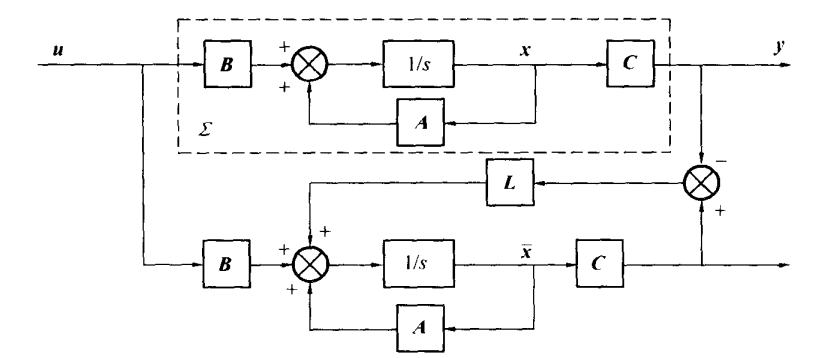
\includegraphics[width=0.7\textwidth]{全维观测器.png}
                \caption{全维观测器的结构图}
            \end{figure}

            全维状态观测器的动态方程$\bm{\dot{\bar x}}=\bm{A\bar x}+\bm{Bu}+\bm{L}(\bm{C\bar x}-\bm{y}),\bm{\bar x}(\bm{0})=\bm{\bar x}_0$

            由$\bm{\dot{\tilde x}}=(\bm{A}+\bm{LC})\bm{\tilde x}$得观测器存在条件是$\bm{A}+\bm{LC}$是渐进稳定的矩阵，称此矩阵对$(\bm{A,C})$是可检测的。

            线性定常系统可检测的充要条件是其对偶系统是可稳的，即对所有不能观振型均具有负实部。

            {\setlength{\parindent}{0pt}\textbf{全维观测器的设计}}
            \begin{itemize}
                \item $[\bm{A}\quad\bm{C}]$可检测：
                \begin{itemize}
                    \item 导出对偶系统$(\bm{A^T,C^T,B^T})$
                    \item 利用线性系统镇定算法求取$\bm{K}$使得$\bm{A^T}+\bm{C^TK}$渐近稳定，即特征值均具有负实部。
                    \item 取$\bm{L}=\bm{K^T}$，计算矩阵$\bm{A}+\bm{LC}$得到全维状态观测器。
                    \end{itemize}
                \item $[\bm{A}\quad\bm{C}]$可观测：
                \begin{itemize}
                    \item 导出对偶系统$(\bm{A^T,C^T,B^T})$
                    \item 指定所要设计的一组期望的极点$\{\lambda^*_i\}$，利用极点配置问题算法用矩阵对$[\bm{A^T\quad C^T}]$确定使$\lambda_i(\bm{A}+\bm{bk})=\lambda_i^*$成立的反馈增益矩阵$\bm{K}$
                    \item 取$\bm{L}=\bm{K^T}$，计算矩阵$\bm{A}+\bm{LC}$得到全维状态观测器。
                \end{itemize}
            \end{itemize}
        \subsubsection{降维状态观测器}
            考虑到系统输出包含状态的部分信息，利用这些信息可以构造出维数低于原系统的状态观测器。可以由输出各分量线性表示的状态分量不必要由状态观测器进行重构。
            若线性定常系统$[\bm{A\quad C}]$是可观测的且$\bm{C}$为满秩矩阵，${\rm rank}\bm{C}=m$，则降维观测器的最小维数为$n-m$

            假设$[\bm{A\quad C}]$可观测，${\rm rank}\bm{C}=m$，选取$(n-m)\times n$阶常阵$\bm{R}$使得$\bm{P}=\begin{bmatrix}\bm{C}\\ \bm{R}\end{bmatrix}$非奇异。
            则$\bm{PP^{-1}}=\bm{I}$，故$\bm{CP^{-1}}=[\bm{I}_{m\times m}\quad\bm{0}]_{m\times n}$
            以$\bm{P}$为变换阵进行代数等价变换得$\bm{\bar A}=\bm{PAP^{-1}}=\begin{bmatrix}\bm{\bar A}_{11}&\bm{\bar A}_{12}\\\bm{\bar A}_{21}&\bm{\bar A}_{22}\end{bmatrix}$，
            $\bm{\bar B}=\bm{PB}=\begin{bmatrix}\bm{\bar B}_1\\ \bm{\bar B}_2\end{bmatrix},\bm{\bar C}=\bm{CP}=[\bm{I}_{m\times m}\quad\bm{0}]$

            变换后系统可以写为
            \[
            \begin{cases}
                \bm{\dot{\bar x}}_1=\bm{\bar A_{11}\bar x_1}+\bm{\bar A_{12}\bar x_2}+\bm{\bar B_{1}u}\\
                \bm{\dot{\bar x}}_2=\bm{\bar A_{21}\bar x_1}+\bm{\bar A_{22}\bar x_2}+\bm{\bar B_{2}u}
            \end{cases}\qquad
            \bm{y}=\bm{\bar c\bar x}=\bm{\bar x_1}
            \]

            因此$\bm{\bar x_1}$是可以直接测量的量，只需要设计$\bm{\bar x_2}$子系统的全维观测器即可。

            将$\bm{y}=\bm{\bar x_1}$代入$\bm{\bar x_1}$子系统状态方程并和$\bm{\bar x_2}$子系统的状态方程整理可得：
            $\bm{\bar A_{12}\bar x_2}=\bm{\dot y}-\bm{\bar A_{11}\bar x_1}-\bm{\bar B_1u}\triangleq\bm{\omega}$

            以$\bm{\omega}$为$\bm{\bar x_2}$子系统的输出设计全维观测器即可。

            $\bm{\dot z}=\bm{\bar A_{22}z}+\bm{\bar A_{21}y}+\bm{\bar B_2u}+\bm{\bar L}(mb{\dot{\bar \omega}}-\bm{\omega})=
            (\bm{\bar A_{22}}+\bm{\bar L\bar A_{12}})\bm{z}+\bm{\bar A_{21}y}+\bm{\bar B_2u}-\bm{\bar L}(\bm{\dot y}-\bm{\bar A_{11}y}-\bm{\bar B_1u})$

            引入$\bm{\bar z}=\bm{z}+\bm{\bar Ly}$以消去$\bm{y}$的导数项，代入整理得：
            $\bm{\dot{\bar z}}=\bm{\dot z}+\bm{L\dot y}=(\bm{\bar A_{22}}+\bm{\bar L\bar A_{12}})\bm{\bar z}+
            [(\bm{\bar A_{21}}+\bm{\bar L\bar A_{11}})-(\bm{\bar A_{22}}+\bm{\bar L\bar A_{12}})\bm{\bar L}]\bm{y}+(\bm{\bar B_2}+\bm{\bar L\bar B_1})\bm{u}$

            $\bm{\bar x_2}$重构状态为$\bm{z}=\bm{\bar z}-\bm{\bar Ly}$，则$\bm{\bar x}$的重构状态为$\bm{\hat{\bar x}}=\begin{bmatrix}\bm{y}\\ \bm{z}-\bm{\bar Ly}\end{bmatrix}$
            因此系统的重构状态$\bm{\hat x}=\bm{P^{-1}\bar x}=\bm{Q\bar x}=\bm{Q_1y}+\bm{Q_2}(\bm{z}-\bm{\bar Ly})=\bm{Q_2z}+(\bm{Q_1}-\bm{\bar L})\bm{y}$
            
            {\setlength{\parindent}{0pt}\textbf{线性系统降维观测器的设计}}

            \begin{itemize}
                \item 选取$(n-m)\times n$阶常阵$\bm{R}$使得$\bm{P}=\begin{bmatrix}\bm{C}\\ \bm{R}\end{bmatrix}$非奇异。
                \item 计算$\bm{Q}=\bm{P}^{-1}=[\bm{Q_1\quad Q_2}]$，其中$\bm{Q_1,Q_2}$分别为$n\times m,n\times(n-m)$维矩阵。
                \item 计算$\bm{\bar A}=\bm{PAP^{-1}}=\begin{bmatrix}\bm{\bar A}_{11}&\bm{\bar A}_{12}\\\bm{\bar A}_{21}&\bm{\bar A}_{22}\end{bmatrix}$，
                $\bm{\bar B}=\bm{PB}=\begin{bmatrix}\bm{\bar B}_1\\ \bm{\bar B}_2\end{bmatrix}$，
                其中$\bm{\bar A}_{11},\bm{\bar A}_{12},\bm{\bar A}_{21},\bm{\bar A}_{22}$分别为$m\times m,m\times (n-m),(n-m)\times m,(n-m)\times(n-m)$阶矩阵，
                $\bm{\bar B}_1,\bm{\bar B}_2$分别为$m\times r,(n-m)\times r$阶矩阵
                \item 选取$\bm{\bar L}$使得$\bm{\bar A}_{22}+\bm{\bar L\bar A}_{12}$稳定或具有$n-m$个希望的极点。
                \item 按照$\bm{\hat x}=\bm{P^{-1}\bar x}=\bm{Q\bar x}=\bm{Q_1y}+\bm{Q_2}(\bm{z}-\bm{\bar Ly})=\bm{Q_2z}+(\bm{Q_1}-\bm{\bar L})\bm{y}$构建降维状态观测器。
            \end{itemize}
    \subsection{解耦问题}
        又称互不影响控制、一对一控制，设计目的是消除输入输出的关联耦合作用，实现每一个输出仅受相应的一个输入控制，每一个输入也仅能控制一个相应的输出。解耦问题前提条件是输入输出变量个数相同。

        若系统的传递函数矩阵$\bm{G}(s)={\rm diag}[g_{11}(s)\quad g_{22}(s)\quad\cdots\quad g_{mm}(s)]$，则该系统是解耦的，此时可以被看做是一组相互独立的单变量系统，实现自治控制。
        \subsubsection{频域的串联动态补偿器解耦}
            \begin{figure}[H]
                \centering
                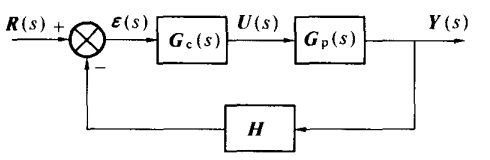
\includegraphics{串联补偿解耦.png}
                \caption{含串联补偿器的解耦系统}
            \end{figure}

            系统闭环传递函数矩阵$\bm{\Phi}(s)=[\bm{I}-\bm{G_p}(s)\bm{G_c}(s)]^{-1}\bm{G_p}(s)\bm{G_c}(s)$
            
            解得串联补偿器的传递函数矩阵$\bm{G_c}(s)=\bm{G_p}^{-1}(s)\bm{\Phi}(s)[\bm{I}-\bm{H}\bm{\Phi}(s)]^{-1}$
        \subsubsection{时域的状态反馈解耦} 
            线性定常系统传递函数$\bm{G}(s)=\bm{C}(s\bm{I}-\bm{A})^{-1}\bm{B}$，进行状态反馈$\bm{u}=\bm{Fx}+\bm{Hr}$，得闭环系统的状态方程为
            \[
            \begin{cases}
            \bm{\dot x}=(\bm{A}+\bm{BF})\bm{x}+\bm{BHr}\\
            \bm{y}=\bm{Cx}
            \end{cases}
            \]
            目的是使得闭环传递函数$\bm{\Phi}(s)=\bm{C}[s\bm{I}-(\bm{A}+\bm{BF})]^{-1}\bm{BH}$变为${\rm diag}\bigg[\frac{1}{s^{d_i+1}}\bigg]$的形式，
            其中$d_i=\min\limits_{j}[\deg Q_{ij}(s)-\deg P_{ij}(s)]-1$为解耦指数。

            设$\bm{c}_i$为系统输出矩阵$\bm{C}$中的第$i$行向量，根据$d_i$定义下列矩阵：
            \[
            \bm{D}=\begin{bmatrix}\bm{c_1A}^{d_1}\\\bm{c_2A}^{d_2}\\\vdots\\\bm{c_m A}^{d_m}\end{bmatrix}\qquad
            \bm{E}=\bm{DB}=\begin{bmatrix}\bm{c_1A}^{d_1}\bm{B}\\\bm{c_2A}^{d_2}\bm{B}\\\vdots\\\bm{c_m A}^{d_m}\bm{B}\end{bmatrix}\qquad
            \bm{L}=\bm{DA}=\begin{bmatrix}\bm{c_1A}^{d_1+1}\\\bm{c_2A}^{d_2+1}\\\vdots\\\bm{c_m A}^{d_m+1}\end{bmatrix}\qquad
            \]

            线性定常系统采用状态反馈能解耦的充要条件是$m\times m$维矩阵$\bm E$是非奇异的，即$\det\bm{E}\neq0$。

            若系统是状态反馈能解耦的，则闭环系统是一个积分型解耦系统，状态反馈矩阵$\bm{F}=-\bm{E^{-1}L}$，输入变换矩阵$\bm{H}=\bm{E}^{-1}$
\end{document}